\documentclass[a4paper,10pt]{article}
\linespread{1.5}
\setlength{\columnseprule}{1pt}
\def\columnseprulecolor{\color{black}}
\usepackage[utf8]{inputenc}
\usepackage[T1]{fontenc}
\usepackage{amsmath}
\usepackage{amsfonts}
\usepackage{amssymb}
\usepackage{mathrsfs}
%\usepackage{mathtools}
\usepackage{rotating}
\usepackage[font=bf]{caption}
\usepackage[nottoc]{tocbibind}
\usepackage{enumitem}
\usepackage{cancel}
\usepackage{xcolor}
\usepackage{graphicx}
\usepackage{wrapfig}
\usepackage{caption}
\usepackage{subcaption}
\usepackage{float}
\floatstyle{boxed}
%\restylefloat{figure}
%\graphicspath{ {/home/ericc/spaces/extspace/molec_dyn/molecular_dynamics_model/paper/} }
\graphicspath{ {./paper/} }
\usepackage[margin=0.254\textwidth]{geometry}
\usepackage{array,tabularx}
\usepackage{listings}
\usepackage{ragged2e}
\usepackage{wasysym}
\usepackage{lipsum}
\usepackage{setspace}
\usepackage{pdfpages}
\usepackage{chemfig}
\usepackage{bohr}

\setbohr{
	electron-options-set = {black!50!black!50}
}

\definecolor{backcolour}{rgb}{0.22,0.22,0.22}
\renewcommand{\ttdefault}{pcr}

\lstdefinestyle{mystyle}{
	backgroundcolor=\color{backcolour},   
	commentstyle=\color{red},
	keywordstyle=\color{green},
	numberstyle=\small\color{gray},
	stringstyle=\color{yellow},
	basicstyle=\ttfamily\bfseries\footnotesize\color{white},
	breakatwhitespace=false,         
	breaklines=true,                 
	captionpos=b,                    
	keepspaces=true,                 
	numbers=left,                    
	numbersep=4pt,                  
	showspaces=false,                
	showstringspaces=false,
	showtabs=false,                  
	tabsize=4,
	language=Python
}
\lstset{style=mystyle}

\newenvironment{tightcenter}{%
  \setlength\topsep{0pt}
  \setlength\parskip{0pt}
  \begin{center}
}{%
  \end{center}
}
%\usepackage{xcolor}  
%\pagecolor[rgb]{0.13,0.17,0.14}  
%\color[rgb]{1,1,1} 

\author{Eric A. Chapman}
\date{\today}
\title{\textbf{Independent Approach to Molecular Dynamics Model Using DNA Encoded Amino Acids with Goal of Simulating Short Peptides to Proteins}}
\author{Eric A. Chapman}
\date{\today}

\begin{document}
\maketitle
\begin{center}
	\textbf{Declaration}
\end{center}
All figures and plots presented in this paper were produced by myself using the python code in the appendix or presentation making software. Of course; unless any figures are cited, referenced or stated otherwise.
\begin{flushright}
	\footnotesize
	\textit{
	- \textbf{Eric A. Chapman}\\
	\today}
\end{flushright}
\begin{center}
	\textbf{Abstract}
\end{center}
to be done at some point
\newpage
\tableofcontents
\listoffigures
\listoftables
\newpage
\section{Introduction -}

\section{Mathematics -}
\subsection{Geometry -}
\subsubsection{Line Intersecting an '\textit{n}'-dimensional sphere -}
In Cartesian coordinates the generalised equation for a circle with an arbitrary origin is as such:
\begin{equation}
\left( x - x_0 \right)^2 + \left( y - y_0 \right)^2 = \rho^2
\end{equation}
But for generality we cannot use the $x_0$ notation used above to denote the origin coordinates. Thus, we shall say these are elements of a wider vector of $n$ length/dimension, and each element counts as a coordinate. We shall therefore call this vector $\underline{\omega}$. We shall also treat $x$ and $y$ and so on in the same way by saying these are part of a vector which we shall label $\underline{r}$. Then for the inside of the brackets above to match up with new vector notation, we need simply subtract $\underline{\omega}$ from $\underline{r}$. Then take the dot product with itself, which looks as such:
\begin{equation}
\rho^2 = (\underline{r}-\underline{\omega}) \cdot (\underline{r}-\underline{\omega})
\end{equation}
Which for convenience we shall change the above notation be like so:
\begin{equation}
	\rho^2 = (\underline{r}-\underline{\omega})^{\cdot 2}
\end{equation}
Next, instead of our nice and simple two dimensional line of $y = mx + c$, we need to use a parametric form to have a line in higher dimensions. Like the $+c$ being an offset for the 2D line, we generalise the offsets for each axis in a vector $\underline{\delta}$. We will also assume that the $x$, $y$, $z$... components are a function of some parameter $t$ with each dimension having some gradient $m_i$ for the $i$th direction. Which we shall also keep in a vector labelled $\underline{m}$. Thus for each dimension, we have equations of the form:
\begin{equation}
x_i = m_i t - \delta_i \ \ \Leftrightarrow \ \ t = \frac{x_i + \delta_i}{m_i}
\end{equation}
Then for the last bit of housekeeping, the above $x_i$ will be the elements of the $\underline{r}$ vector that corresponds to the points of the line.

We can then substitute this into the previous equation that we have for a generalised sphere, which gives us:
\begin{equation}
\rho^2 = (\underline{m} t - \underline{\delta} - \underline{\omega})^{\cdot 2}
\end{equation}
\begin{equation}
	\rho^2 = \underline{m}^{\cdot 2} t^2 - 2  \underline{m} \cdot (\underline{\delta} + \underline{\omega}) t + \underline{\delta}^{\cdot 2} + \underline{\omega}^{\cdot 2} + 2 \underline{\delta} \cdot \underline{\omega}
\end{equation}
Then letting:
\begin{equation}
\varphi_a = \underline{m}^{\cdot 2}
\end{equation}
\begin{equation}
\varphi_b = \underline{m} \cdot (\underline{\delta} + \underline{\omega})
\end{equation}
\begin{equation}
\varphi_c = \underline{\delta}^{\cdot 2} + \underline{\omega}^{\cdot 2} + 2 \underline{\delta} \cdot \underline{\omega} - \rho^2
\end{equation}
\begin{equation}
\Rightarrow \ \ 0 = \varphi_a t^2 - 2\varphi_b t + \varphi_c
\end{equation}
The above can then be used to gain the two values of $t$ via use of the quadratic formula, which keeping the '$-2$' in the equation above makes the formula somewhat nicer to use.
\begin{equation}
t = \frac{1}{\varphi_a} \left(\varphi_b \pm \sqrt{\varphi_b^2 - \varphi_a \varphi_c} \right)
\end{equation}
$$ \Rightarrow \ \ t = t^\pm $$

\section{The Natural Amino Acids -}
\rule{\textwidth}{1pt}
\subsection{What We Will be Looking At -}
In total, there are twenty such amino acids that are produced from DNA encoding. These are encoded as such:
\begin{figure}[H]
\centering
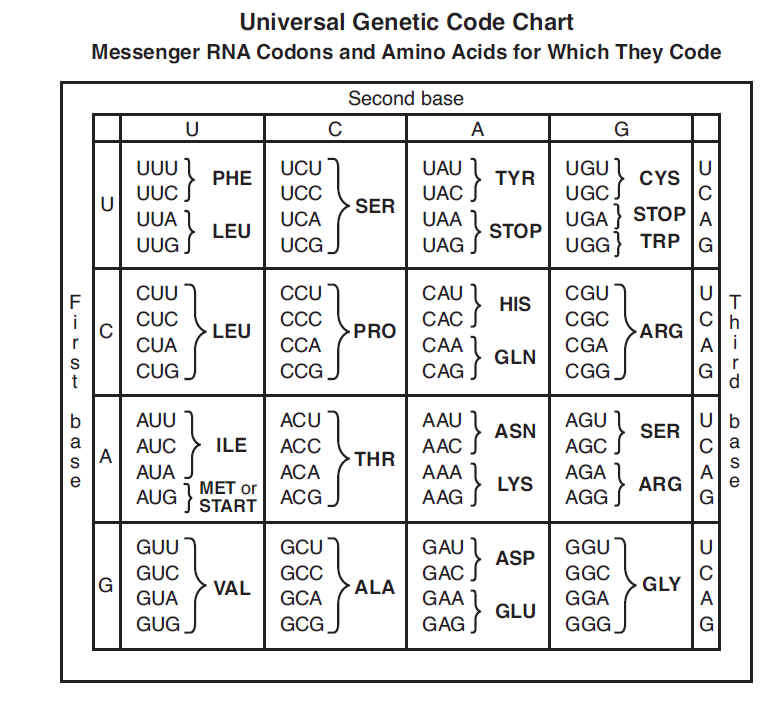
\includegraphics[width=0.6\textwidth]{images/rna_ecode.png}
\caption{Encoding of Amino Acids to RNA Bases}
\label{fig:rna_chart}
\end{figure}
One will notice that the above corresponds to RNA encoding (UCAG) which uses \textit{uracil}, \textit{cytosine}, \textit{adenine} and \textit{guanine}. For the above to use the nucleotides (or bases) that DNA uses, all one would have to do is swap uracil for \textit{thymine}, i.e. 'U' for 'T'. Thus also to give names to the three letter codes that one will see in the chart above, do have a look at \textbf{Table \ref{tab:tnaa} \cite{chart}}. 

We shall then -in the proceeding subsection- go through and see the two 2-dimensional structures that the represent these molecules. These two representations being the structural and skeletal formulae. After that we shall discuss how to turn these in to some form of data structure that preserves chirality, implicit structure and gives what could be the start of a mapping in coordinate space.

\begin{table}[h!]
\captionsetup{justification=centering}
\noindent\makebox[\textwidth]{%
\centering
\small
\begin{tabular}{|r|c|c|c|}
\hline
 & \textbf{Amino Acid} & \textbf{3 Letter Code} & \textbf{1 Letter Code} \\
\hline
1 & Alanine & Ala & A\\
2 & Arginine & Arg & R\\
3 & Asparagine & Asn & N\\
4 & Aspartic Acid & Asp & D\\
5 & Cysteine & Cys & C\\
6 & Glutamine & Gln & Q\\
7 & Glutamic Acid & Glu & E\\
8 & Glycine & Gly & G\\
9 & Histidine & His & H\\
10 & Isoleucine & Ile & I\\
11 & Leucine & Leu & L\\
12 & Lysine & Lys & K\\
13 & Methionine & Met & M\\
14 & Phenylalanine & Phe & F\\
15 & Proline & Pro & P\\
16 & Serine & Ser & S\\
17 & Threonine & Thr & T\\
18 & Tryptophan & Trp & W\\
19 & Tyrosine & Tyr & Y\\
20 & Valine & Val & V\\
\hline
\end{tabular}
}
\caption{\small{The 20 Natural Amino Acids with Their 3 \& 1 Letter Codes}}
\label{tab:tnaa}
\end{table}




\section{Turning Structural Formulae into Tables -}
\rule{\textwidth}{1pt}
\subsection{Rules to Turn into Table -}
Right, so now we shall endeavour to build some data structure or framework where we can represent the structural formulae (as that shows all elements present in the molecule) as some form of table. We shall first suppose the two bond structures that we will most certainly see. Those being tetrahedral and trigonal which look like so:

\begin{minipage}{0.5\textwidth}
\subsubsection{Tetrahedral -}
\begin{center}
\small{
\chemfig{{\left[ 0 \right]}(-[::+0]{\left[ 3 \right]})(-[::+90]{\left[ 2 \right]})(-[::+180]{\left[ 1 \right]})(-[::-90]{\left[ 4 \right]})}
}
\end{center}
\end{minipage}%
\begin{minipage}{0.5\textwidth}
\subsubsection{Trigonal Planar -}
\begin{center}
\small{
\chemfig{{\left[ 0 \right]}(-[::-30]{\left[ 3 \right]})(-[::+90]{\left[ 2 \right]})(-[::+210]{\left[ 1 \right]})}
}
\end{center}
\end{minipage}\newline\bigskip

Now from looking at the above, there are at most five elements in and around the central element (depicted as $[0]$) we can therefore say that the table will have five columns. Suppose we have the following two cases:\newline\bigskip

\begin{minipage}{0.5\textwidth}
\begin{center}
\small{
\chemfig{C(-[::+0]H)(-[::+90]C)(-[::+180]C)(-[::-90]N)}
}
\end{center}
\end{minipage}%
\begin{minipage}{0.5\textwidth}
\begin{center}
\small{
\chemfig{C(-[::+30]O)(=[::+150]O)(-[::+270]C)}
}
\end{center}
\end{minipage}\newline\bigskip

Where one may recognise the right hand example to be similar to the carbon found amongst a carboxylic acid group and left to what we will soon refer to as the 'central' carbon of a given amino acid. So how would the above translate to their allocated 'row' within a table. Well, the tetrahedral case would look as such:

\begin{table}[h!]
\captionsetup{justification=centering}
\noindent\makebox[\textwidth]{%
\centering
\small
\begin{tabular}{|r|ccccc|}
\hline
Path/Bond Index & 0 & 1 & 2 & 3 & 4 \\
\hline
0 & C & -C & -C & -H & -N \\
\hline
\end{tabular}
}
\caption{\small{Example of Tetrahedral Table Row}}
\label{tab:btetr}
\end{table}

\begin{table}[h!]
\captionsetup{justification=centering}
\noindent\makebox[\textwidth]{%
\centering
\small
\begin{tabular}{|r|ccccc|}
\hline
Path/Bond Index & 0 & 1 & 2 & 3 & 4 \\
\hline
0 & C & =O & -O & -C & X \\
\hline
\end{tabular}
}
\caption{\small{Example of Trigonal Table Row}}
\label{tab:btrir}
\end{table}

Here we can see that to interpret the table, one must accept a \textit{rule of end-points}. In other words, we need to use 'X' as the identifier of a trigonal bonding around the atom in question of that row and is therefore an end point. Plus, in terms of what an atom can be bonded to, we must add '=O' and '-H' to the list of end points. It is best now to do this, not just for one row of the table but for an entire molecule, and so we shall construct the table for alanine. Recalling the structure that was presented earlier, to make the table, we will first need to present its structure in a more fuller fashion. i.e.

\begin{center}
\footnotesize{
\chemfig{C(-[::+0]H)(-[::+90]C(=[::+60]O)(-[::-60] O (-[::+0]H)))(-[::-90]N(-[::-90]H)(-[::+0]H))(-[::+180] H \chembelow{\chemabove{C}{H}}{H})}}
\end{center}

\begin{center}
\bohr{16}{O} \bohr{14}{N}
\end{center}

\subsection{Preserving Correct Chirality -}



\newpage
\begin{appendix}
\section{Structural, Skeletal Formulae \& Structure Tables -}
\rule{\textwidth}{1pt}
\subsection{Alanine -}
{
\begin{minipage}{0.5\textwidth}
\begin{center}
\footnotesize{
\chemfig{C(-[::+0]H)(-[::+90]C(=[::+60]O)(-[::-60]OH))(-[::-90]N(-[::-90]H)(-[::+0]H))(-[::+180]H_3 C)}
}
\end{center}
\end{minipage}%
\begin{minipage}{0.5\textwidth}
\begin{center}
\small{
\chemfig{(-[::+30](=[::+60]O)-[::-60]OH)(<[::-90]N H_2)(-[::+150]H_3 C)}
}
\end{center}
\end{minipage}
}

\begin{table}[h!]
\captionsetup{justification=centering}
\noindent\makebox[\textwidth]{%
\centering
\small
\begin{tabular}{|l|ccccc|}
\hline
 & [0] & [1] & [2] & [3] & [4]\\
\hline
0 & C & -C & -C & -H & -N\\
01 & C & -H & -H & -C & -H\\
02 & C & =O & -O & -C & X\\
04 & N & -H & -C & ee & -H\\
022 & O & -H & ee & ee & -C\\
\hline
\end{tabular}
}
\caption{\small{Alanine Structure Table}}
\label{tab:ala}
\end{table}


\subsection{Arginine -}
{
\begin{minipage}{0.5\textwidth}
\begin{center}
\footnotesize{
\chemfig{
C(-[::+0]H)(-[::+90]C(=[::+60]O)(-[::-60]OH))(-[::-90]N(-[::-90]H)(-[::+0]H))(-[::+180]{\left({CH}_{2}\right)}_{3}-[::+0]N(-[::+90]H)-[::+0]C(=[::-90]NH)-[::+0]H_{2} N)}
}
\end{center}
\end{minipage}%
\begin{minipage}{0.5\textwidth}
\begin{center}
\small{
\chemfig{(-[::+30](=[::+60]O)-[::-60]OH)(<[::-90]N H_2)(-[::+150]-[::+60]-[::-60]-[::+60]\chembelow{N}{H}-[::-60](=[::-60]NH)-[::+60]{H_2}N)}
}
\end{center}
\end{minipage}
}

\begin{table}[h!]
\captionsetup{justification=centering}
\noindent\makebox[\textwidth]{%
\centering
\small
\begin{tabular}{|l|ccccc|}
\hline
 & [0] & [1] & [2] & [3] & [4]\\
\hline
0 & C & -C & -C & -H & -N\\
01 & C & -C & -H & -C & -H\\
02 & C & =O & -O & -C & X\\
04 & N & -H & -C & ee & -H\\
011 & C & -C & -H & -C & -H\\
022 & O & -H & ee & ee & -C\\
0111 & C & -N & -H & -C & -H\\
01111 & N & -H & ee & -C & -H\\
011111 & C & -N & =N & -N & X\\
0111111 & N & -H & ee & -C & -H\\
0111112 & N & -H & ee & =C & X\\\hline
\end{tabular}
}
\caption{\small{Arginine Structure Table}}
\label{tab:arg}
\end{table}


\subsection{Asparagine -}
{
\begin{minipage}{0.5\textwidth}
\begin{center}
\footnotesize{
\chemfig{C(-[::+0]H)(-[::+90]C(=[::+60]O)(-[::-60]OH))(-[::-90]N(-[::-90]H)(-[::+0]H))(-[::+180]CH_2 -[::+0]C(=[::-60]O)-[::+60]H_2 N)}
}
\end{center}
\end{minipage}%
\begin{minipage}{0.5\textwidth}
\begin{center}
\small{
\chemfig{(-[::+30](=[::+60]O)-[::-60]OH)(<[::-90]N H_2)(-[::+150]-[::+60](=[::+60]O)-[::-60]H_2 N)}
}
\end{center}
\end{minipage}
}

\begin{table}[h!]
\captionsetup{justification=centering}
\noindent\makebox[\textwidth]{%
\centering
\small
\begin{tabular}{|l|ccccc|}
\hline
 & [0] & [1] & [2] & [3] & [4]\\
\hline
0 & C & -C & -C & -H & -N\\
01 & C & -C & -H & -C & -H\\
02 & C & =O & -O & -C & X\\
04 & N & -H & -C & ee & -H\\
011 & C & -N & =O & -C & X\\
022 & O & -H & ee & ee & -C\\
0111 & N & -H & ee & -C & -H\\
\hline
\end{tabular}
}
\caption{\small{Asparagine Structure Table}}
\label{tab:asn}
\end{table}


\subsection{Aspartic Acid -}
{
\begin{minipage}{0.5\textwidth}
\begin{center}
\footnotesize{
\chemfig{C(-[::+0]H)(-[::+90]C(=[::+60]O)(-[::-60]OH))(-[::-90]N(-[::-90]H)(-[::+0]H))(-[::+180]CH_2 -[::+0]C(=[::-60]O)-[::+60]HO)}
}
\end{center}
\end{minipage}%
\begin{minipage}{0.5\textwidth}
\begin{center}
\small{
\chemfig{(-[::+30](=[::+60]O)-[::-60]OH)(<[::-90]N H_2)(-[::+150]-[::+60](=[::+60]O)-[::-60]HO)}
}
\end{center}
\end{minipage}
}

\begin{table}[h!]
\captionsetup{justification=centering}
\noindent\makebox[\textwidth]{%
\centering
\small
\begin{tabular}{|l|ccccc|}
\hline
 & [0] & [1] & [2] & [3] & [4]\\
\hline
0 & C & -C & -C & -H & -N\\
01 & C & -C & -H & -C & -H\\
02 & C & =O & -O & -C & X\\
04 & N & -H & -C & ee & -H\\
011 & C & -O & =O & -C & X\\
022 & O & -H & ee & ee & -C\\
0111 & O & -H & -C & ee & ee\\
\hline
\end{tabular}
}
\caption{\small{Aspartic Acid Structure Table}}
\label{tab:asp}
\end{table}


\subsection{Cysteine -}
{
\begin{minipage}{0.5\textwidth}
\begin{center}
\footnotesize{
\chemfig{C(-[::+0]H)(-[::+90]C(=[::+60]O)(-[::-60]OH))(-[::-90]N(-[::-90]H)(-[::+0]H))(-[::+180]CH_2-[::+0]HS)}
}
\end{center}
\end{minipage}%
\begin{minipage}{0.5\textwidth}
\begin{center}
\small{
\chemfig{(-[::+30](=[::+60]O)-[::-60]OH)(<[::-90]N H_2)(-[::+150]-[::+60]HS)}
}
\end{center}
\end{minipage}
}

\begin{table}[h!]
\captionsetup{justification=centering}
\noindent\makebox[\textwidth]{%
\centering
\small
\begin{tabular}{|l|ccccc|}
\hline
 & [0] & [1] & [2] & [3] & [4]\\
\hline
0 & C & -C & -C & -H & -N\\
01 & C & -S & -H & -C & -H\\
02 & C & =O & -O & -C & X\\
04 & N & -H & -C & ee & -H\\
011 & S & -H & ee & -C & ee\\
022 & O & -H & ee & ee & -C\\
\hline
\end{tabular}
}
\caption{\small{Cysteine Structure Table}}
\label{tab:cys}
\end{table}


\subsection{Glutamine -}
{
\begin{minipage}{0.5\textwidth}
\begin{center}
\footnotesize{
\chemfig{C(-[::+0]H)(-[::+90]C(=[::+60]O)(-[::-60]OH))(-[::-90]N(-[::-90]H)(-[::+0]H))(-[::+180]{\left({CH}_{2}\right)}_{2} -[::+0]C(=[::-60]O)-[::+60]H_2 N)}
}
\end{center}
\end{minipage}%
\begin{minipage}{0.5\textwidth}
\begin{center}
\small{
\chemfig{(-[::+30](=[::+60]O)-[::-60]OH)(<[::-90]N H_2)(-[::+150]-[::+60]-[::-60](=[::-60]O)-[::+60]H_2 N)}
}
\end{center}
\end{minipage}
}

\begin{table}[h!]
\captionsetup{justification=centering}
\noindent\makebox[\textwidth]{%
\centering
\small
\begin{tabular}{|l|ccccc|}
\hline
 & [0] & [1] & [2] & [3] & [4]\\
\hline
0 & C & -C & -C & -H & -N\\
01 & C & -C & -H & -C & -H\\
02 & C & =O & -O & -C & X\\
04 & N & -H & -C & ee & -H\\
011 & C & -C & -H & -C & -H\\
022 & O & -H & ee & ee & -C\\
0111 & C & -N & =O & -C & X\\
01111 & N & -H & ee & -C & -H\\
\hline
\end{tabular}
}
\caption{\small{Glutamine Structure Table}}
\label{tab:gln}
\end{table}


\subsection{Glutamic Acid -}
{
\begin{minipage}{0.5\textwidth}
\begin{center}
\footnotesize{
\chemfig{C(-[::+0]H)(-[::+90]C(=[::+60]O)(-[::-60]OH))(-[::-90]N(-[::-90]H)(-[::+0]H))(-[::+180]{\left({CH}_{2}\right)}_{2} -[::+0]C(=[::-60]O)-[::+60]HO)}
}
\end{center}
\end{minipage}%
\begin{minipage}{0.5\textwidth}
\begin{center}
\small{
\chemfig{(-[::+30](=[::+60]O)-[::-60]OH)(<[::-90]N H_2)(-[::+150]-[::+60]-[::-60](=[::-60]O)-[::+60]HO)}
}
\end{center}
\end{minipage}
}

\begin{table}[h!]
\captionsetup{justification=centering}
\noindent\makebox[\textwidth]{%
\centering
\small
\begin{tabular}{|l|ccccc|}
\hline
 & [0] & [1] & [2] & [3] & [4]\\
\hline
0 & C & -C & -C & -H & -N\\
01 & C & -C & -H & -C & -H\\
02 & C & =O & -O & -C & X\\
04 & N & -H & -C & ee & -H\\
011 & C & -C & -H & -C & -H\\
022 & O & -H & ee & ee & -C\\
0111 & C & -O & =O & -C & X\\
01111 & O & -H & -C & ee & ee\\
\hline
\end{tabular}
}
\caption{\small{Glutamic Acid Structure Table}}
\label{tab:glu}
\end{table}


\subsection{Glycine -}
{
\begin{minipage}{0.5\textwidth}
\begin{center}
\footnotesize{
\chemfig{C(-[::+0]H)(-[::+90]C(=[::+60]O)(-[::-60]OH))(-[::-90]N(-[::-90]H)(-[::+0]H))(-[::+180]H)}
}
\end{center}
\end{minipage}%
\begin{minipage}{0.5\textwidth}
\begin{center}
\small{
\chemfig{(-[::+30](=[::+60]O)-[::-60]OH)(<[::-90]N H_2)}
}
\end{center}
\end{minipage}
}

\begin{table}[h!]
\captionsetup{justification=centering}
\noindent\makebox[\textwidth]{%
\centering
\small
\begin{tabular}{|l|ccccc|}
\hline
 & [0] & [1] & [2] & [3] & [4]\\
\hline
0 & C & -H & -C & -H & -N\\
02 & C & =O & -O & -C & X\\
04 & N & -H & -C & ee & -H\\
022 & O & -H & ee & ee & -C\\
\hline
\end{tabular}
}
\caption{\small{Glycine Structure Table}}
\label{tab:gly}
\end{table}


\subsection{Histidine -}
{
\begin{minipage}{0.5\textwidth}
\begin{center}
\footnotesize{
\chemfig{C(-[::+0]H)(-[::+90]C(=[::+60]O)(-[::-60]OH))(-[::-90]N(-[::-90]H)(-[::+0]H))(-[::+180]CH_2 -[::+0]C*5(-N=C(-[::-54]H)-N(-[::-54]H)-C(-[::-54]H)=))}
}
\end{center}
\end{minipage}%
\begin{minipage}{0.5\textwidth}
\begin{center}
\small{
\chemfig{(-[::+30](=[::+60]O)-[::-60]OH)(<[::-90]N H_2)(-[::+150]-[::+60]*5(-N=-\chembelow{N}{H}-=))}
}
\end{center}
\end{minipage}
}

\begin{table}[h!]
\captionsetup{justification=centering}
\noindent\makebox[\textwidth]{%
\centering
\small
\begin{tabular}{|l|ccccc|}
\hline
 & [0] & [1] & [2] & [3] & [4]\\
\hline
0 & C & -C & -C & -H & -N\\
01 & C & -C & -H & -C & -H\\
02 & C & =O & -O & -C & X\\
04 & N & -H & -C & ee & -H\\
011 & C & =C & -N & -C & X\\
022 & O & -H & ee & ee & -C\\
0111 & C & -N & =C & -H & X\\
0112 & N & =C & ee & -C & X\\
01111 & N & ee & -H & -C & -C\\
01121 & C & -H & =N & -N & X\\
\hline
\end{tabular}
}
\caption{\small{Histidine Structure Table}}
\label{tab:his}
\end{table}


\subsection{Isoleucine -}
{
\begin{minipage}{0.5\textwidth}
\begin{center}
\footnotesize{
\chemfig{C(-[::+0]H)(-[::+90]C(=[::+60]O)(-[::-60]OH))(-[::-90]N(-[::-90]H)(-[::+0]H))(-[::+180]CH(-[::-90]CH_3)-[::+0]CH_2 -[::+0]H_3 C)}
}
\end{center}
\end{minipage}%
\begin{minipage}{0.5\textwidth}
\begin{center}
\small{
\chemfig{(-[::+30](=[::+60]O)-[::-60]OH)(<[::-90]N H_2)(-[::+150](<:[::-60]CH_3)-[::+60]-[::-60]H_3 C)}
}
\end{center}
\end{minipage}
}

\begin{table}[h!]
\captionsetup{justification=centering}
\noindent\makebox[\textwidth]{%
\centering
\small
\begin{tabular}{|l|ccccc|}
\hline
 & [0] & [1] & [2] & [3] & [4]\\
\hline
0 & C & -C & -C & -H & -N\\
01 & C & -C & -C & -C & -H\\
02 & C & =O & -O & -C & X\\
04 & N & -H & -C & ee & -H\\
011 & C & -C & -H & -C & -H\\
012 & C & -H & -H & -H & -C\\
022 & O & -H & ee & ee & -C\\
0111 & C & -H & -H & -C & -H\\
\hline
\end{tabular}
}
\caption{\small{Isoleucine Structure Table}}
\label{tab:ile}
\end{table}


\subsection{Leucine -}
{
\begin{minipage}{0.5\textwidth}
\begin{center}
\footnotesize{
\chemfig{C(-[::+0]H)(-[::+90]C(=[::+60]O)(-[::-60]OH))(-[::-90]N(-[::-90]H)(-[::+0]H))(-[::+180]CH_2-[::+0]C(-[::+90]CH_3)(-[::-90]H)(-[::+0]H_3 C))}
}
\end{center}
\end{minipage}%
\begin{minipage}{0.5\textwidth}
\begin{center}
\small{
\chemfig{(-[::+30](=[::+60]O)-[::-60]OH)(<[::-90]N H_2)(-[::+150]-[::+60](-[::+60]CH_3)-[::-60]H_3 C)}
}
\end{center}
\end{minipage}
}

\begin{table}[h!]
\captionsetup{justification=centering}
\noindent\makebox[\textwidth]{%
\centering
\small
\begin{tabular}{|l|ccccc|}
\hline
 & [0] & [1] & [2] & [3] & [4]\\
\hline
0 & C & -C & -C & -H & -N\\
01 & C & -C & -H & -C & -H\\
02 & C & =O & -O & -C & X\\
04 & N & -H & -C & ee & -H\\
011 & C & -C & -H & -C & -C\\
022 & O & -H & ee & ee & -C\\
0111 & C & -H & -H & -C & -H\\
0114 & C & -H & -C & -H & -H\\
\hline
\end{tabular}
}
\caption{\small{Leucine Structure Table}}
\label{tab:leu}
\end{table}


\subsection{Lysine -}
{
\begin{minipage}{0.5\textwidth}
\begin{center}
\footnotesize{
\chemfig{C(-[::+0]H)(-[::+90]C(=[::+60]O)(-[::-60]OH))(-[::-90]N(-[::-90]H)(-[::+0]H))(-[::+180]{\left( CH_2 \right)}_{4} -[::+0]H_2 N)}
}
\end{center}
\end{minipage}%
\begin{minipage}{0.5\textwidth}
\begin{center}
\small{
\chemfig{(-[::+30](=[::+60]O)-[::-60]OH)(<[::-90]N H_2)(-[::+150]-[::+60]-[::-60]-[::+60]-[::-60] H_2 N)}
}
\end{center}
\end{minipage}
}

\begin{table}[h!]
\captionsetup{justification=centering}
\noindent\makebox[\textwidth]{%
\centering
\small
\begin{tabular}{|l|ccccc|}
\hline
 & [0] & [1] & [2] & [3] & [4]\\
\hline
0 & C & -C & -C & -H & -N\\
01 & C & -C & -H & -C & -H\\
02 & C & =O & -O & -C & X\\
04 & N & -H & -C & ee & -H\\
011 & C & -C & -H & -C & -H\\
022 & O & -H & ee & ee & -C\\
0111 & C & -C & -H & -C & -H\\
01111 & C & -N & -H & -C & -H\\
011111 & N & -H & ee & -C & -H\\
\hline
\end{tabular}
}
\caption{\small{Lysine Structure Table}}
\label{tab:lys}
\end{table}


\subsection{Methionine -}
{
\begin{minipage}{0.5\textwidth}
\begin{center}
\footnotesize{
\chemfig{C(-[::+0]H)(-[::+90]C(=[::+60]O)(-[::-60]OH))(-[::-90]N(-[::-90]H)(-[::+0]H))(-[::+180]{\left( CH_2 \right)}_{2} -[::+0]S-[::+0]H_3 C)}
}
\end{center}
\end{minipage}%
\begin{minipage}{0.5\textwidth}
\begin{center}
\small{
\chemfig{(-[::+30](=[::+60]O)-[::-60]OH)(<[::-90]N H_2)(-[::+150]-[::+60]-[::-60]S-[::+60]H_3 C)}
}
\end{center}
\end{minipage}
}

\begin{table}[h!]
\captionsetup{justification=centering}
\noindent\makebox[\textwidth]{%
\centering
\small
\begin{tabular}{|l|ccccc|}
\hline
 & [0] & [1] & [2] & [3] & [4]\\
\hline
0 & C & -C & -C & -H & -N\\
01 & C & -C & -H & -C & -H\\
02 & C & =O & -O & -C & X\\
04 & N & -H & -C & ee & -H\\
011 & C & -S & -H & -C & -H\\
022 & O & -H & ee & ee & -C\\
0111 & S & -C & ee & -C & ee\\
01111 & C & -H & -H & -C & -H\\
\hline
\end{tabular}
}
\caption{\small{Methionine Structure Table}}
\label{tab:met}
\end{table}


\subsection{Phenylalanine -}
{
\begin{minipage}{0.5\textwidth}
\begin{center}
\footnotesize{
\chemfig{C(-[::+0]H)(-[::+90]C(=[::+60]O)(-[::-60]OH))(-[::-90]N(-[::-90]H)(-[::+0]H))(-[::+180]CH_2-[::+0]C**6(-C(-[::-60]H)-C(-[::-60]H)-C(-[::-60]H)-C(-[::-60]H)-C(-[::-60]H)-))}
}
\end{center}
\end{minipage}%
\begin{minipage}{0.5\textwidth}
\begin{center}
\small{
\chemfig{(-[::+30](=[::+60]O)-[::-60]OH)(<[::-90]N H_2)(-[::+150]-[::+60]**6(------))}
}
\end{center}
\end{minipage}
}

\begin{table}[h!]
\captionsetup{justification=centering}
\noindent\makebox[\textwidth]{%
\centering
\small
\begin{tabular}{|l|ccccc|}
\hline
 & [0] & [1] & [2] & [3] & [4]\\
\hline
0 & C & -C & -C & -H & -N\\
01 & C & -C & -H & -C & -H\\
02 & C & =O & -O & -C & X\\
04 & N & -H & -C & ee & -H\\
011 & C & -C & =C & -C & X\\
022 & O & -H & ee & ee & -C\\
0111 & C & =C & -C & -H & X\\
0112 & C & -C & -H & =C & X\\
01111 & C & -H & -C & =C & X\\
01121 & C & =C & -H & -C & X\\
011112 & C & -H & =C & -C & X\\
\hline
\end{tabular}
}
\caption{\small{Phenylalanine Structure Table}}
\label{tab:phe}
\end{table}


\subsection{Proline -}
{
\begin{minipage}{0.5\textwidth}
\begin{center}
\footnotesize{
\chemfig{C(-[::+0]H)(-[::+90]C(=[::+60]O)(-[::-60]OH))([::-145]*5(-\chemabove{C}{H_2} -H_2 C -\chembelow{C}{H_2} -\chembelow{N}{H}-))}
}
\end{center}
\end{minipage}%
\begin{minipage}{0.5\textwidth}
\begin{center}
\small{
\chemfig{(([::+180]*5(----NH>))-[::+30](=[::+60]O)-[::-60]OH)}
}
\end{center}
\end{minipage}
}

\begin{table}[h!]
\captionsetup{justification=centering}
\noindent\makebox[\textwidth]{%
\centering
\small
\begin{tabular}{|l|ccccc|}
\hline
 & [0] & [1] & [2] & [3] & [4]\\
\hline
0 & C & -C & -C & -H & -N\\
01 & C & -H & -H & -C & -C\\
02 & C & =O & -O & -C & X\\
04 & N & -C & -C & ee & -H\\
014 & C & -H & -H & -C & -C\\
022 & O & -H & ee & ee & -C\\
041 & C & -H & -C & -N & -H\\
0144 & C & -H & -C & -C & -H\\
\hline
\end{tabular}
}
\caption{\small{Proline Structure Table}}
\label{tab:pro}
\end{table}


\subsection{Serine -}
{
\begin{minipage}{0.5\textwidth}
\begin{center}
\footnotesize{
\chemfig{C(-[::+0]H)(-[::+90]C(=[::+60]O)(-[::-60]OH))(-[::-90]N(-[::-90]H)(-[::+0]H))(-[::+180]CH_2 -[::+0]HO)}
}
\end{center}
\end{minipage}%
\begin{minipage}{0.5\textwidth}
\begin{center}
\small{
\chemfig{(-[::+30](=[::+60]O)-[::-60]OH)(<[::-90]N H_2)(-[::+150]-[::+60]HO)}
}
\end{center}
\end{minipage}
}

\begin{table}[h!]
\captionsetup{justification=centering}
\noindent\makebox[\textwidth]{%
\centering
\small
\begin{tabular}{|l|ccccc|}
\hline
 & [0] & [1] & [2] & [3] & [4]\\
\hline
0 & C & -C & -C & -H & -N\\
01 & C & -O & -H & -C & -H\\
02 & C & =O & -O & -C & X\\
04 & N & -H & -C & ee & -H\\
011 & O & -H & ee & -C & ee\\
022 & O & -H & ee & ee & -C\\
\hline
\end{tabular}
}
\caption{\small{Serine Structure Table}}
\label{tab:ser}
\end{table}


\subsection{Threonine -}
{
\begin{minipage}{0.5\textwidth}
\begin{center}
\footnotesize{
\chemfig{C(-[::+0]H)(-[::+90]C(=[::+60]O)(-[::-60]OH))(-[::-90]N(-[::-90]H)(-[::+0]H))(-[::+180]CH(-[::-90]OH)-[::+0]H_3 C)}
}
\end{center}
\end{minipage}%
\begin{minipage}{0.5\textwidth}
\begin{center}
\small{
\chemfig{(-[::+30](=[::+60]O)-[::-60]OH)(<[::-90]N H_2)(-[::+150](<[::-60]OH)-[::+60]H_3 C)}
}
\end{center}
\end{minipage}
}

\begin{table}[h!]
\captionsetup{justification=centering}
\noindent\makebox[\textwidth]{%
\centering
\small
\begin{tabular}{|l|ccccc|}
\hline
 & [0] & [1] & [2] & [3] & [4]\\
\hline
0 & C & -C & -C & -H & -N\\
01 & C & -C & -O & -C & -H\\
02 & C & =O & -O & -C & X\\
04 & N & -H & -C & ee & -H\\
011 & C & -H & -H & -C & -H\\
012 & O & ee & -H & ee & -C\\
022 & O & -H & ee & ee & -C\\
\hline
\end{tabular}
}
\caption{\small{Threonine Structure Table}}
\label{tab:thr}
\end{table}


\subsection{Tryptophan -}
{
\begin{minipage}{0.5\textwidth}
\begin{center}
\footnotesize{
\chemfig{C(-[::+0]H)(-[::+90]C(=[::+60]O)(-[::-60]OH))(-[::-90]N(-[::-90]H)(-[::+0]H))(-[::+180]CH_2 -[::+0]C*5(=C(-[::-54]H)-N(-[::-54]H)-C*6(-C(-[::-60]H)=C(-[::-60]H)-C(-[::-60]H)=C(-[::-60]H)-C=)-C-))}
}
\end{center}
\end{minipage}%
\begin{minipage}{0.5\textwidth}
\begin{center}
\small{
\chemfig{(-[::+30](=[::+60]O)-[::-60]OH)(<[::-90]N H_2)(-[::+150]-[::+60] *5(-*6(-=-=-=)--\chembelow{N}{H}-=))}
}
\end{center}
\end{minipage}
}

\begin{table}[h!]
\captionsetup{justification=centering}
\noindent\makebox[\textwidth]{%
\centering
\small
\begin{tabular}{|l|ccccc|}
\hline
 & [0] & [1] & [2] & [3] & [4]\\
\hline
0 & C & -C & -C & -H & -N\\
01 & C & -C & -H & -C & -H\\
02 & C & =O & -O & -C & X\\
04 & N & -H & -C & ee & -H\\
011 & C & -C & =C & -C & X\\
022 & O & -H & ee & ee & -C\\
0111 & C & =C & -C & -C & X\\
0112 & C & -N & -H & =C & X\\
01121 & N & -H & ee & -C & -C\\
01111 & C & -C & -N & =C & X\\
01113 & C & =C & -C & -H & X\\
011111 & C & -H & -C & =C & X\\
011131 & C & -C & =C & -H & X\\
0111113 & C & -H & =C & -C & X\\
\hline
\end{tabular}
}
\caption{\small{Tryptophan Structure Table}}
\label{tab:trp}
\end{table}


\subsection{Tyrosine -}
{
\begin{minipage}{0.5\textwidth}
\begin{center}
\footnotesize{
\chemfig{C(-[::+0]H)(-[::+90]C(=[::+60]O)(-[::-60]OH))(-[::-90]N(-[::-90]H)(-[::+0]H))(-[::+180]CH_2-[::+0]C**6(-C(-[::-60]H)-C(-[::-60]H)-C(-[::-60]HO)-C(-[::-60]H)-C(-[::-60]H)-))}
}
\end{center}
\end{minipage}%
\begin{minipage}{0.5\textwidth}
\begin{center}
\small{
\chemfig{(-[::+30](=[::+60]O)-[::-60]OH)(<[::-90]N H_2)(-[::+150]-[::+60]**6(---(-[::-60]HO)---))}
}
\end{center}
\end{minipage}
}

\begin{table}[h!]
\captionsetup{justification=centering}
\noindent\makebox[\textwidth]{%
\centering
\small
\begin{tabular}{|l|ccccc|}
\hline
 & [0] & [1] & [2] & [3] & [4]\\
\hline
0 & C & -C & -C & -H & -N\\
01 & C & -C & -H & -C & -H\\
02 & C & =O & -O & -C & X\\
04 & N & -H & -C & ee & -H\\
011 & C & -C & =C & -C & X\\
022 & O & -H & ee & ee & -C\\
0111 & C & =C & -C & -H & X\\
0112 & C & -C & -H & =C & X\\
01111 & C & -H & -C & =C & X\\
01121 & C & =C & -H & -C & X\\
011112 & C & -O & =C & -C & X\\
0111121 & O & -H & ee & -C & ee\\
\hline
\end{tabular}
}
\caption{\small{Tyrosine Structure Table}}
\label{tab:tnaa}
\end{table}tyr

\subsection{Valine -}
{
\begin{minipage}{0.5\textwidth}
\begin{center}
\footnotesize{
\chemfig{C(-[::+0]H)(-[::+90]C(=[::+60]O)(-[::-60]OH))(-[::-90]N(-[::-90]H)(-[::+0]H))(-[::+180]CH(-[::-90]CH_3)-[::+0]H_3 C)}
}
\end{center}
\end{minipage}%
\begin{minipage}{0.5\textwidth}
\begin{center}
\small{
\chemfig{(-[::+30](=[::+60]O)-[::-60]OH)(<[::-90]N H_2)(-[::+150](-[::-60]CH_3)-[::+60]H_3 C)}
}
\end{center}
\end{minipage}
}

\begin{table}[h!]
\captionsetup{justification=centering}
\noindent\makebox[\textwidth]{%
\centering
\small
\begin{tabular}{|l|ccccc|}
\hline
 & [0] & [1] & [2] & [3] & [4]\\
\hline
0 & C & -C & -C & -H & -N\\
01 & C & -C & -C & -C & -H\\
02 & C & =O & -O & -C & X\\
04 & N & -H & -C & ee & -H\\
011 & C & -H & -H & -C & -H\\
012 & C & -H & -H & -H & -C\\
022 & O & -H & ee & ee & -C\\
\hline
\end{tabular}
}
\caption{\small{Valine Structure Table}}
\label{tab:val}
\end{table}

\end{appendix}

\newpage
\begin{thebibliography}{10}

\bibitem{chart}
	"Transcription vs Translation." Diffen.com. Diffen LLC, n.d. Web. 28 May 2021. < https://www.diffen.com/difference/Transcription\textunderscore vs\textunderscore Translation >
\bibitem{example}
	Authors. Year of Publish. \textit{Title}. edition/printing. City of publish: printing office/press.
\end{thebibliography}

\end{document}
